\clearpage
\section[Fully-coupled model]{Solving a problem using a Fully-Coupled Model}\label{tutorial-coupled}

The process of solving a problem using \Dumux can be roughly divided into four parts:
\begin{enumerate}
 \item The geometry of the problem and correspondingly a grid have to be defined.
 \item Material properties and constitutive relationships have to be defined.
 \item Boundary conditions as well as initial conditions have to be defined.
 \item A suitable model has to be chosen.
\end{enumerate}

The problem that is solved in this tutorial is illustrated in figure \ref{tutorial-coupled:problemfigure}. A rectangular domain with no flow boundaries on the top and on the bottom, which is initially saturated with oil, is considered. Water infiltrates from the left side into the domain. Gravity effects as well as capillarity effects are neglected.

\begin{figure}[h]
\psfrag{x}{x}
\psfrag{y}{y}
\psfrag{no flow}{no flow}
\psfrag{water}{\textbf{water}}
\psfrag{oil}{\textcolor{white}{\textbf{oil}}}
\psfrag{p_w = 2 x 10^5 [Pa]}{$p_w = 2 \times 10^5$ [Pa]}
\psfrag{p_w_initial = 2 x 10^5 [Pa]}{\textcolor{white}{\textbf{$\mathbf{p_{w_{initial}} = 2 \times 10^5}$ [Pa]}}}
\psfrag{S_n = 0}{$S_n = 0$}
\psfrag{S_n_initial = 0}{\textcolor{white}{$\mathbf{S_{n_{initial}} = 1}$}}
\psfrag{q_w = 0 [kg/m^2s]}{$q_w = 0$ $\left[\frac{\textnormal{kg}}{\textnormal{m}^2 \textnormal{s}}\right]$}
\psfrag{q_n = -3 x 10^-4 [kg/m^2s]}{$q_n = -3 \times 10^-4$ $\left[\frac{\textnormal{kg}}{\textnormal{m}^2 \textnormal{s}}\right]$}
\centering
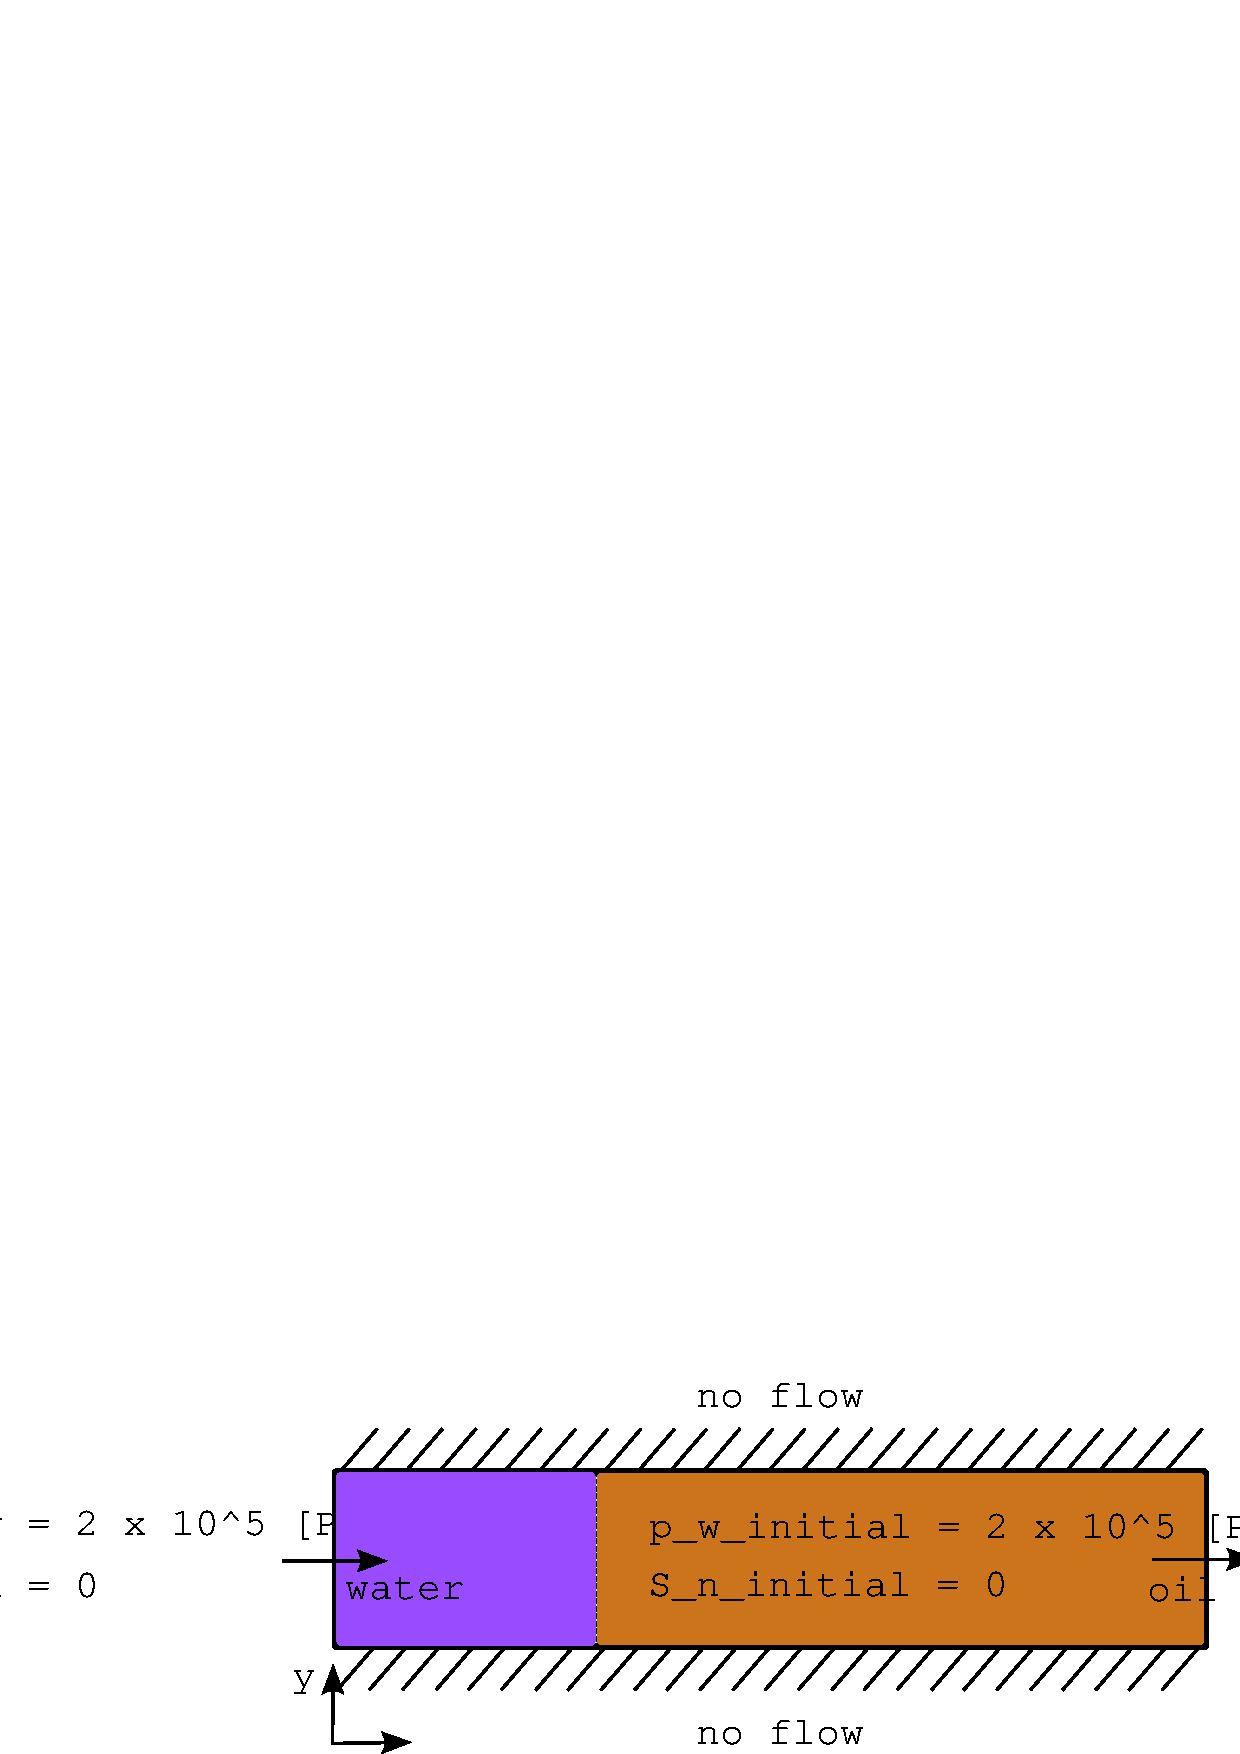
\includegraphics[width=0.9\linewidth,keepaspectratio]{EPS/tutorial-problemconfiguration}
\caption{Geometry of the tutorial problem with initial and boundary conditions.}\label{tutorial-coupled:problemfigure}
\end{figure}

Listing \ref{tutorial-coupled:mainfile} shows the main file \texttt{tutorial\_coupled.cc} for the coupled twophase model. This file needs to be executed to solve the problem described above. The main file can be found in the directory \texttt{/dune-mux/test/tutorial}.

\begin{lst}[File dune-mux/test/tutorial/tutorial\_coupled.cc]\label{tutorial-coupled:mainfile} \mbox{}
\lstinputlisting[basicstyle=\ttfamily\scriptsize,numbers=left,
numberstyle=\tiny, numbersep=5pt]{../../test/tutorial/tutorial_coupled.cc}
\end{lst}

From line \ref{tutorial-coupled:include-begin} to line \ref{tutorial-coupled:include-end} the Dune and the \Dumux files which contain the functions and classes that are needed in the main function are included into the main file.

The geometry of the problem and the grid on which the problem is to be solved are defined in the lines \ref{tutorial-coupled:grid-begin} to \ref{tutorial-coupled:grid-end}. The three variables of Type \texttt{Dune::FieldVector} define the lower left corner of the domain (\texttt{L}), the upper right corner of the domain (\texttt{H}) and the number of cells in $x$ and $y$ direction (\texttt{N}). The dimension \texttt{dim} is previously defined in line \ref{tutorial-coupled:dim}. The grid of type \texttt{Dune::SGrid} is then generated in line \ref{tutorial-coupled:grid-end}. For more information about the dune grid interface, the different grid types that are supported and the generation of different grids it is referred to the \textit{Dune Grid Interface HOWTO (http://www.dune-project.org/doc/)}.

The second step needed to solve the problem is the definition of material properties and constitutive relationships. The fluid properties of the two fluid phases considered here are defined in the lines \ref{tutorial-coupled:water} and \ref{tutorial-coupled:oil}. \Dumux provides several fluid classes which can be found in the file \texttt{phaseproperties2p.hh} in the directory \texttt{/dune-mux/dumux}-\texttt{/material/phaseproperties}. \\
The properties of the solid matrix are defined in a special soil class. The \texttt{soil} object is generated in line \ref{tutorial-coupled:soil}. As can be seen, the class type is \texttt{Dune::TutorialSoil}, which is defined in the file \texttt{tutorial\_soilproperties.hh} in the folder \texttt{/test/tutorial}. A description of this file and the definition of a soil class including the soil parameters can be found in section \ref{tutorial-coupled:description-soil-class}. Finally, in line \ref{tutorial-coupled:twophaserelations} the information included in the fluid and soil objects is used to generate an object of type \texttt{Dune::TwoPhaseRelations}, which includes the constitutive relationships (capillary pressure-saturation relation, relative permeability-saturation relation, etc.). The file \texttt{twophaserelations.hh} can be found in the directory \texttt{/dune-mux/dumux/material}.

The definition of boundary and initial conditions as well as source or sink terms is done by definition of a so-called \textit{problem} class. In case of this tutorial the problem class is defined in the file \texttt{tutorialproblem\_coupled.hh} in the \texttt{/test/tutorial} folder. In the main file the problem object of type \texttt{Dune::TutorialProblemCoupled} is then generated in line \ref{tutorial-coupled:problem}. A further explanation of the definition of boundary and initial conditions, source and sink terms and the structure of the problem class can be found in section \ref{tutorial-coupled:description-bc-ic}. Besides the definition of the boundary and initial conditions the problem class is also a kind of interface containing all the objects generated before (geometry, fluids, soil, constitutive relationships, etc.). Thus, as can be seen in line \ref{tutorial-coupled:problem} all this objects are given as arguments when calling the constructor of the problem class.     

Finally, a numerical model has to be chosen that defines how the coupled system of equations is discretized. In case of this tutorial a coupled isothermal two phase model is the choice. A coupled model may consist of two or more mass balance equations and if required an energy balance equation. For the given example problem of a pure isothermal two phase flow. A coupled system of two equations is solved. 
%The two equations are given below:
%\begin{equation}
%\end{equation}
%GLEICHUNGEN\\
%ERKLAERUNG ZU BOX\\

The discretisation of these equations is included in the object which is generated in line \ref{tutorial-coupled:boxmethod} of the main file. It is called \texttt{boxmethod} and it is of type \texttt{Dune::BoxPwSn}. The definition of this class can be found in \texttt{/dune-mux/dumux/twophase/fv} in the file \texttt{boxpwsnjacobian.hh}. The \texttt{Box} in the class name indicates that the \textit{boxmethod} is used for the discretisation. 

Finally, an object called \texttt{timeloop} of type \texttt{Dune::TimeLoop} is generated in line \ref{tutorial-coupled:timeloop} of the tutorial main file. The class \texttt{Dune::TimeLoop} is defined in the file \texttt{timeloop.hh} in the folder \texttt{/dune-mux/dumux/timedisc}. The object \texttt{timeloop} includes the type of timestep that is used (implicit, explicit, etc.) and contains the function \texttt{execute} which is called in line \ref{tutorial-coupled:execute} of the main file. This function finally starts the computation and runs the (time)loop over all timesteps.

\subsection{The definition of the fluid properties}\label{tutorial-coupled:description-fluid-class}

In \Dumux different fluids are already implemented. The definitions can be found in the file \texttt{phaseproperties2p.hh} in the directory \texttt{/dune-mux/dumux/material/phaseproperties}. In this file, for each fluid a class named like the fluid is defined. These classes are derived from the fluid base class \texttt{Fluid} which is defined in the file \texttt{property\_baseclasses.hh} in the directory \texttt{/dune-mux/dumux/material} and include several functions returning different fluid properties. New fluids which are not yet available in the file \texttt{phaseproperties2p.hh} can be defined here accordingly.

It is important to mention, that existing fluid classes should not be changed. New fluid classes should only be added to the file \texttt{phaseproperties2p.hh} if they are also to be added to the repository! If you are not sure if your fluid class can be useful for the other \Dumux users just create a new file in your problem directory similar to the file \texttt{phaseproperties2p.hh} and define your fluid classes there.

\subsection{The definition of the soil parameters}\label{tutorial-decoupled:description-soil-class}

Soil properties which can be defined in \Dumux are the \textit{intrinsic permeability}, the \textit{porosity} and the \textit{heat capacity} as well as the \textit{heat conductivity} of the solid matrix. Further the \textit{residual saturations} of the fluids, and the \textit{capillary pressures-saturation function} as well as the \textit{relative permeability-saturation functions} are depending on the soil.

The base class \texttt{Dune::Matrix2p} for the definition of the soil parameters can be found in the file \texttt{property\_baseclasses.hh} in the directory \texttt{/dune-mux/dumux/material}. Derived from this base class, there exist two standard soil type classes named \texttt{HomogeneousSoil} and \texttt{HeterogeneousSoil}. Both can be found in the file \texttt{matrixproperties.hh} in the \texttt{/material} folder. If one wants to use a soil that differs from this standard soil types, new soil classes can be derived either from the base class (\texttt{Dune::Matrix2p}) or from the two standard soil classes (\texttt{Dune::HomogeneousSoil} and \texttt{Dune::HeterogeneousSoil}).

For this tutorial problem a new soil class named \texttt{TutorialSoil} is derived from \texttt{Dune::HomogeneousSoil} (listing \ref{tutorial-decoupled:soilpropertiesfile}, line \ref{tutorial-decoupled:tutorialsoil}), which can be found in the file \texttt{tutorial\_soilproperties.hh} in the directory \texttt{/test/tutorial}.

Listing \ref{tutorial-decoupled:soilpropertiesfile} shows the file \texttt{tutorial\_soilproperties.hh}.

\begin{lst}[File dune-mux/test/tutorial/tutorial\_soilproperties.hh]\label{tutorial-decoupled:soilpropertiesfile} \mbox{}
\lstinputlisting[basicstyle=\ttfamily\scriptsize,numbers=left,
numberstyle=\tiny, numbersep=5pt]{../../test/tutorial/tutorial_soilproperties.hh}
\end{lst}

In line \ref{tutorial-decoupled:permeability} the function returning the intrinsic permeability can be found. As can be seen, the function has to be called with three different arguments. The first one (\texttt{x}) is a vector including the global coordinates of the current entity (can be an element, vertex, etc.), the second one (\texttt{e}) is the entity itself and the third one is a vector including the local coordinates of the current entity. The intrinsic permeability is a tensor and thus returned in form of a $n \times n$-matrix where $n$ is the dimension of the problem.

The function \texttt{porosity()} defined in line \ref{tutorial-decoupled:porosity} is called with the same arguments as the permeability function described before and returns the porosity dependent on the position in the domain.

The residual saturation functions \texttt{Sr\_w()} (line \ref{tutorial-decoupled:srw}) and \texttt{Sr\_n()} (line \ref{tutorial-decoupled:srn}) additionally have the temperature as function argument, which is set to a default value if an isothermal model is used.

Finally, the functions defining the type of the capillary pressure function and the relative permeability functions have to be considered. In line \ref{tutorial-decoupled:flags} the function \texttt{relPermFlag()} is defined. This function returns a flag indicating the type of function which is used depending on the position. This could be a linear function, a \textit{Brooks-Corey} function, a \textit{van Genuchten} function, etc. The flags that can be chosen as return parameter are defined in the base soil class \texttt{Matrix2p} in the file \texttt{property\_baseclasses.hh}. The parameters used in the chosen function type can be defined in the function \texttt{paramRelPerm} (line \ref{tutorial-decoupled:parameters}). As can be seen in listing \ref{tutorial-decoupled:soilpropertiesfile}, e.g. linear capillary pressure and relative permeability functions require a vector of two arguments, one defining the minimum and one defining the maximum capillary pressure. The parameters can again be defined depending on the position in the domain an on temperature.

\subsection{The definition of boundary and initial conditions and source or sink terms}\label{tutorial-coupled:description-bc-ic}

Boundary and initial conditions are defined in a so-called problem class. The problem class of this tutorial has the name \texttt{TutorialProblemCoupled} and is defined in the file \texttt{tutorialproblem\_coupled.hh} which can be found in the directory \texttt{/test/tutorial}. Listing \ref{tutorial-coupled:problemfile} shows the class \texttt{TutorialProblemCoupled}. As can be seen it is derived from the problem base class \texttt{TwoPhaseProblem} (line \ref{tutorial-coupled:tutorialproblem}) which is defined in the file \texttt{twophaseproblem.hh} in the directory \texttt{/dune-mux/dumux/twophase}.

\begin{lst}[File dune-mux/test/tutorial/tutorialproblem\_coupled.hh]\label{tutorial-coupled:problemfile} \mbox{}
\lstinputlisting[basicstyle=\ttfamily\scriptsize,numbers=left,
numberstyle=\tiny, numbersep=5pt]{../../test/tutorial/tutorialproblem_coupled.hh}
\end{lst}

Listing \ref{tutorial-coupled:tutorialproblem}) includes five types of functions. The type of each function can be identified by certain letters or names. The function that returns
\begin{itemize}
 \item a source or sink term is called \textbf{q},
 \item a boundary condition type is called \textbf{bctype},
 \item a \textit{Dirichlet} boundary condition is called \textbf{g},
 \item a \textit{Neumann} boundary condition is called \textbf{J} and
 \item an initial condition is called \textbf{initial}.
\end{itemize}

All different function types have to be called with three different argum
ents. The first one (\texttt{x}) is a vector including the global coordin
ates of the current entity (can be an element, vertex, etc.), the second
one (\texttt{e}) is the entity itself and the third one is a vector inclu
ding the local coordinates of the current entity. Thus, the return of the
 functions, which can be a boundary value, an initial value, a source/sin
k, etc., can be defined depending on the position in the domain.

The first function defined in the problem class \texttt{TutorialProblemCoupled} is the function \texttt{q} (line \ref{tutorial-coupled:q}). It returns a source or a sink term for the pressure equation.

In line \ref{tutorial-coupled:bctype} the function returning the boundary condition type is defined. 
Flags of type \\
\texttt{Dune::BoundaryConditions::Flags} have to be used as return value of these functions. 
The flags that can be chosen are defined in the file \texttt{boundaryconditions.hh} in the directory \texttt
{/dune-disc/disc/operators}.

In lines \ref{tutorial-coupled:g} the functions returning the \textit{Dirichlet} boundary condition and
in line \ref{tutorial-coupled:J} a function returning the \textit{Neumann} boundary condition are defined.

Finally, the function \texttt{initial} is defined in line \ref{tutorial-coupled:initial}. This function returns the initial values for the pressure and the
saturation.

\subsection{Exercise}
TODO: give some exercises

